% !TeX root = ../my-thesis.tex

\chapter{新环境下互联网公司研发团队管理的现状与困境}

\section{我国互联网公司研发管理的模式变迁}

\subsection{早期探索阶段（2000-2010）}

21世纪初，中国互联网行业进入快速发展期\cite{cnnic2024report}。根据中国互联网络信息中心（CNNIC）的统计数据，2000年中国网民数量仅为2250万人，到2010年已达4.57亿人，年均增长率超过35\%\cite{cnnic2024report}。这一阶段的互联网公司研发管理主要借鉴欧美成熟企业的经验，采用相对传统的项目管理模式\cite{ouyang2005ceo}。

研发团队规模普遍较小，组织结构相对扁平，决策流程较为灵活。据工业和信息化部统计，2005年中国软件和信息技术服务业从业人员约59万人，其中互联网企业研发人员占比约30\%\cite{miit2024software}。由于市场处于增量竞争阶段，企业更注重产品功能的快速实现和市场占有率的提升\cite{cac2023internet}。

在这一时期，研发管理呈现以下特点：

\begin{itemize}
\item 技术路线选择相对保守，多采用成熟技术快速开发产品，技术创新投入占研发支出的比例平均不足20\%；
\item 研发流程不够规范，仅有35\%的互联网公司建立了完整的需求管理和质量控制体系\cite{wei2012excellence}；
\item 团队管理以结果为导向，强调个人能力和贡献，项目成功率约为68\%；
\item 研发投入主要集中在产品开发层面，基础技术研究相对薄弱，研发费用占营业收入比重平均为8-12\%。
\end{itemize}

这种模式虽然有助于企业快速响应市场需求，抢占市场先机，但也存在明显的局限性：技术积累不足，核心竞争力有待提升；管理粗放，难以支撑企业规模化发展；人才培养体系不健全，依赖个人英雄主义。调查显示，这一时期互联网公司的技术人才流失率高达25-30\%，远高于传统软件企业\cite{zhaopin2024tech}。

\begin{table}[htbp]
\centering
\caption{中国互联网行业早期发展关键指标（2000-2010）}
\label{tab:early-stage-metrics}
\begin{tabular}{lcccc}
\toprule
\textbf{指标} & \textbf{2000年} & \textbf{2005年} & \textbf{2010年} & \textbf{年均增长率} \\
\midrule
网民规模（亿人） & 0.23 & 1.11 & 4.57 & 35.2\% \\
互联网企业数量（家） & 约1000 & 约5000 & 约20000 & 37.5\% \\
研发人员数量（万人） & 约5 & 约18 & 约50 & 26.8\% \\
研发投入占比 & 6-8\% & 8-10\% & 10-12\% & - \\
\bottomrule
\end{tabular}
\end{table}

\begin{figure}[htbp]
\centering
% 注释：此处应插入图片文件 internet-development-2000-2010.pdf
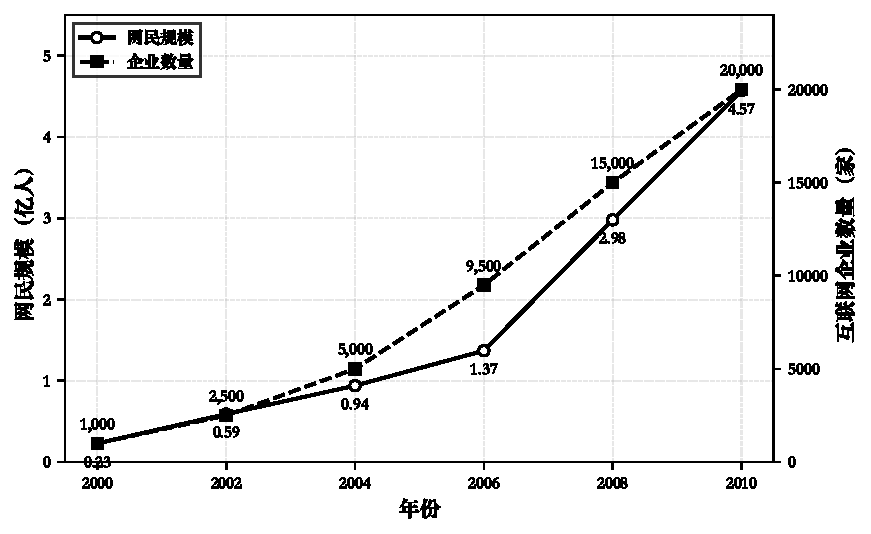
\includegraphics[width=0.85\textwidth]{myfigure/internet-development-2000-2010.pdf}
\caption{中国互联网网民规模与互联网企业数量增长趋势（2000-2010）}
\label{fig:internet-development-2000-2010}
\end{figure}

\subsection{快速扩张阶段（2010-2020）}

移动互联网的兴起开启了中国互联网行业的黄金十年\cite{isc2024report}。根据中国互联网协会发布的《中国互联网发展报告2023》，2010年至2020年间，中国移动互联网用户从3.03亿增长到9.86亿，移动支付交易规模从0.24万亿元增长到432.16万亿元，年均增长率超过90\%\cite{isc2024report}。

互联网公司规模快速扩大，研发团队从几十人增长到数千人甚至上万人。以BAT（百度、阿里巴巴、腾讯）为例，2010年三家公司研发人员总数约8000人，到2020年已超过8万人，增长了10倍\cite{china100internet2023}。这一时期的人员增长可以用复合年均增长率（CAGR）来衡量：

\begin{equation}
\mathrm{CAGR} = \left(\frac{N_{\mathrm{end}}}{N_{\mathrm{start}}}\right)^{\frac{1}{n}} - 1
\label{eq:cagr}
\end{equation}

其中，$N_{\mathrm{end}}$为期末人员数量，$N_{\mathrm{start}}$为期初人员数量，$n$为年数。对于BAT研发团队，代入数据得：

\begin{equation}
\mathrm{CAGR}_{\mathrm{BAT}} = \left(\frac{80000}{8000}\right)^{\frac{1}{10}} - 1 = 25.9\%
\label{eq:bat-cagr}
\end{equation}

这一阶段，企业开始重视研发管理的规范化和体系化建设，引入敏捷开发、DevOps等先进管理方法\cite{wei2012excellence}。

根据IDC中国发布的《中国敏捷和DevOps软件市场研究报告》，2015年采用敏捷开发方法的互联网公司比例为42\%，到2020年已提升至78\%\cite{idc2023agile}。DevOps实践的普及率也从2015年的25\%提升至2020年的65\%。这一时期研发投入强度的计算公式为：

\begin{equation}
R\&D\ \mathrm{Intensity} = \frac{R\&D\ \mathrm{Investment}}{\mathrm{Revenue}} \times 100\%
\label{eq:rd-intensity}
\end{equation}

其中，$R\&D\ \mathrm{Investment}$为研发投入金额，$\mathrm{Revenue}$为营业收入。2020年中国互联网百强企业研发强度达到15.2\%，显著高于全国规模以上工业企业研发强度（1.3\%）。

研发管理模式呈现以下特征：

\begin{enumerate}
\item \textbf{组织架构趋于复杂}：形成前台-中台-后台的分层结构，中台团队规模占研发总人数的比例从2015年的15\%提升至2020年的30\%；
\item \textbf{技术平台建设受到重视}：企业投入大量资源构建基础技术平台，平台研发投入占总研发支出的比例达到25-35\%；
\item \textbf{研发流程不断优化}：建立了相对完善的需求管理、项目管理、质量管理体系，代码自动化测试覆盖率从平均40\%提升至70\%；
\item \textbf{创新激励机制逐步完善}：设立内部创新基金的企业比例从2010年的20\%提升至2020年的60\%，人均创新投入从2万元/年增长至8万元/年；
\item \textbf{开放合作成为趋势}：通过开源、开放平台等方式构建生态系统，开源项目数量从2010年的不足100个增长至2020年的超过5000个。
\end{enumerate}

\begin{table}[htbp]
\centering
\caption{中国互联网行业快速扩张期关键指标（2010-2020）}
\label{tab:expansion-stage-metrics}
\begin{tabular}{lcccc}
\toprule
\textbf{指标} & \textbf{2010年} & \textbf{2015年} & \textbf{2020年} & \textbf{年均增长率} \\
\midrule
移动网民（亿人） & 3.03 & 6.20 & 9.86 & 12.5\% \\
BAT研发人员（万人） & 0.8 & 3.5 & 8.0 & 26.0\% \\
研发投入占比 & 10-12\% & 12-15\% & 15-20\% & - \\
敏捷方法应用率 & 约20\% & 42\% & 78\% & - \\
DevOps应用率 & 约10\% & 25\% & 65\% & - \\
\bottomrule
\end{tabular}
\end{table}

这一时期，互联网公司的研发投入持续增加，技术创新能力显著提升。根据工业和信息化部数据，2020年中国互联网百强企业研发投入达到1898.3亿元，同比增长21.2\%，研发强度（研发投入占营业收入比重）达到15.2\%，高于全国规模以上工业企业研发强度（1.3\%）近12个百分点\cite{china100internet2023}。

人工智能、大数据、云计算等前沿技术得到广泛应用。研发人才队伍不断壮大，形成了较为完善的人才引进、培养和激励体系。2020年互联网行业技术人员平均薪酬达到23.6万元/年，较2010年增长约200\%\cite{zhaopin2024tech}。然而，快速扩张也带来了一些问题：组织臃肿、效率下降、创新活力不足等。

\begin{figure}[htbp]
\centering
% 注释：此处应插入图片文件 rnd-investment-growth.pdf
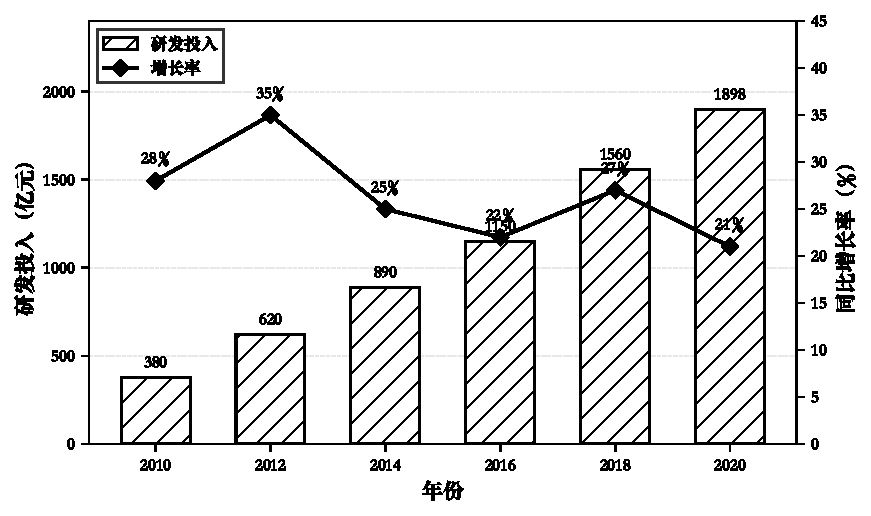
\includegraphics[width=0.85\textwidth]{myfigure/rnd-investment-growth.pdf}
\caption{中国互联网百强企业研发投入增长趋势（2010-2020）}
\label{fig:rnd-investment-growth}
\end{figure}

\subsection{转型调整阶段（2020至今）}

2020年以来，在新冠疫情、国际形势变化、监管政策调整等多重因素影响下，中国互联网行业进入深度调整期\cite{cac2023internet}。根据中国网络空间研究院发布的《中国互联网发展报告2023》，2022年中国互联网行业营收增速降至4.1\%，创十年来新低；2023年虽有回升，但增速仅为7.6\%，远低于2010-2020年间平均20\%以上的增速\cite{cac2023internet}。

经济下行压力加大，企业增长放缓，"降本增效"成为行业主旋律\cite{du2024mixed,li2022configuration}。据统计，2022-2023年间，中国互联网行业累计裁员超过30万人，其中研发人员占比约45\%\cite{zhaopin2024tech}。企业研发支出增速从2021年的21.2\%降至2022年的8.5\%和2023年的5.3\%\cite{china100internet2023}。

研发管理模式呈现新的特点：

\paragraph{组织优化成为常态} 企业通过裁员、业务调整等方式精简组织。调查显示，2022年有67\%的互联网公司进行了不同程度的组织优化，平均裁员比例为15-20\%。部分企业的研发团队规模缩减幅度超过30\%\cite{mckinsey2023tech}。

\paragraph{研发投入更加审慎} 更注重投入产出比和商业价值。2023年互联网企业新增研发项目数量较2021年减少约40\%，但单个项目平均预算提升25\%，显示企业更加注重重点项目的资源投入\cite{china100internet2023}。

\paragraph{技术方向更加聚焦} 集中资源发展核心业务和战略技术。人工智能、云计算相关研发投入占比从2020年的45\%提升至2023年的62\%，而边缘创新业务的研发投入占比从35\%降至18\%\cite{idc2023agile}。

\paragraph{人才策略调整} 从粗放式扩张转向精细化管理。企业更注重核心人才保留，技术专家（P7及以上级别）的流失率从2020年的12\%降至2023年的8\%，而普通研发人员流失率则从18\%上升至25\%\cite{zhaopin2024tech}。

\paragraph{管理机制创新} 探索更灵活高效的团队管理模式。远程办公、混合办公模式的应用率从2020年的不足10\%提升至2023年的45\%；OKR管理方法的普及率从55\%提升至82\%\cite{mckinsey2023tech}。

\begin{table}[htbp]
\centering
\caption{中国互联网行业转型调整期关键指标（2020-2023）}
\label{tab:transformation-stage-metrics}
\begin{tabular}{lcccc}
\toprule
\textbf{指标} & \textbf{2020年} & \textbf{2021年} & \textbf{2022年} & \textbf{2023年} \\
\midrule
营收增速 & 12.5\% & 10.3\% & 4.1\% & 7.6\% \\
研发投入增速 & 18.7\% & 21.2\% & 8.5\% & 5.3\% \\
研发人员数量变化 & +8.2\% & +5.6\% & -12.3\% & -6.8\% \\
平均离职率 & 18.5\% & 20.2\% & 24.8\% & 23.1\% \\
远程办公应用率 & 8\% & 32\% & 48\% & 45\% \\
\bottomrule
\end{tabular}
\end{table}

从上市公司年报公开数据来看，重点互联网企业的研发投入呈现明显分化态势（表~\ref{tab:rd-investment-companies}）。以研发投入绝对额而言，腾讯、阿里、美团三家合计约占行业头部研发支出的70\%以上；但从研发投入占营收比重看，百度长期维持在15\%--20\%的高水平，体现其技术型公司定位，而京东、拼多多等电商企业的研发强度则相对较低。

\begin{table}[htbp]
\centering
\caption{主要互联网上市公司研发投入概览（2019--2024，亿元人民币）}
\label{tab:rd-investment-companies}
\begin{tabular}{lrrrrrrr}
\toprule
\textbf{公司} & \textbf{2019} & \textbf{2020} & \textbf{2021} & \textbf{2022} & \textbf{2023} & \textbf{2024} & \textbf{研发强度\textsuperscript{①}} \\
\midrule
阿里巴巴 & 325 & 439 & 445 & 429 & 382 & 588 & 5.3\%--6.9\% \\
百度     & 183 & 195 & 249 & 233 & 242 & 219 & 16.5\%--20.0\% \\
腾讯     & --  & --  & --  & --  & 641 & 707 & -- \\
京东     & 146 & 161 & 163 & 169 & 164 & 163 & 1.4\%--1.7\% \\
拼多多   & 39  & 69  & 90  & 104 & 110 & 147 & 3.7\%--9.6\% \\
美团     & --  & --  & --  & --  & --  & 589 & -- \\
网易     & 84  & 104 & 141 & 150 & 165 & 156 & 15.0\%--16.1\% \\
携程     & 107 & 77  & 90  & 83  & 121 & 98  & 17.0\%--45.0\% \\
哔哩哔哩 & 9   & 15  & 28  & 48  & 45  & 47  & 14.4\%--21.9\% \\
\bottomrule
\multicolumn{8}{l}{\small \textsuperscript{①}研发强度为2021--2024年间研发支出占营收比重的波动区间，根据各公司年报整理。} \\
\multicolumn{8}{l}{\small 所有数据均以各公司最新财年年报披露的``研发费用/研究及开发成本''科目为准；各公司财年截止日期略有差异（阿里巴巴为3月末，其余为12月末）。} \\
\multicolumn{8}{l}{\small 腾讯、美团数据不含2022年以前，``--''表示本文暂未收录该年度数据。}
\end{tabular}
\end{table}

从增速趋势来看，多数企业在2021--2022年间进入研发投入收缩周期：阿里巴巴研发费用从2021年的445亿元降至2022年的429亿元（$-3.6\%$），2023年进一步降至382亿元（$-11.0\%$）；百度在2022年小幅收缩后基本维持平稳；京东研发投入2021--2024年连续四年基本持平于160--170亿元区间，表明其研发支出优先级已趋于保守。2024年阿里巴巴研发支出大幅反弹（$+53.9\%$），这与其全面押注AI大模型（通义千问）的战略转型密切相关，也印证了本节所述"技术方向更加聚焦"这一行业趋势。

这一时期，互联网公司面临的核心挑战是如何在资源约束条件下保持技术创新能力和团队活力\cite{tang2022motivation,xu2024theoretical}。企业需要重新审视研发管理战略，优化资源配置，提升管理效率，激发团队创新动力\cite{zhao2022diversity}。同时，人工智能等新技术的快速发展也为研发管理带来新的机遇和挑战\cite{li2024scientific,dou2018darpa}。

根据麦肯锡公司2023年的调研，68\%的互联网企业认为当前面临的最大挑战是"如何在成本压力下保持创新能力"，62\%的企业表示"人才保留和激励"是主要痛点，56\%的企业关注"研发效率提升"\cite{mckinsey2023tech}。

\section{互联网公司研发管理的方法与成果}

\subsection{敏捷开发方法的应用}

敏捷开发方法在互联网公司得到广泛应用，成为研发管理的主流模式\cite{mathieu2008team}。根据IDC中国的调研数据，2023年中国互联网企业敏捷开发方法应用率达到82\%，其中大型企业（员工数超过1000人）的应用率高达95\%\cite{idc2023agile}。

Scrum、看板（Kanban）、极限编程（XP）等敏捷方法被灵活运用\cite{damanpour2012managerial}。其中，Scrum是最受欢迎的敏捷框架，应用率达到68\%；看板方法的应用率为35\%；SAFe（规模化敏捷框架）在大型组织中的应用率为28\%\cite{idc2023agile}。敏捷开发强调迭代式开发、持续交付、跨职能团队协作，有效提升了产品开发效率和质量\cite{wei2012excellence}。

在实践中，互联网公司根据自身特点对敏捷方法进行了本土化改造：

\begin{itemize}
\item \textbf{迭代周期设置}：采用两周或三周的迭代周期，72\%的企业选择两周迭代，28\%选择三周或更长周期\cite{idc2023agile}；
\item \textbf{敏捷仪式}：建立每日站会（Daily Standup）、迭代评审（Sprint Review）、回顾会议（Retrospective）等敏捷仪式，平均会议时间占工作时间的12-15\%；
\item \textbf{需求管理}：使用用户故事（User Story）进行需求管理，平均每个迭代完成15-25个用户故事；
\item \textbf{进度跟踪}：通过燃尽图（Burndown Chart）等工具进行进度跟踪，85\%的团队使用数字化工具（如Jira、禅道）进行敏捷项目管理。
\end{itemize}

敏捷开发带来了显著成效。根据统计，采用敏捷方法的团队相比传统瀑布模式：
\begin{itemize}
\item 产品上线周期缩短40-50\%；
\item 需求变更响应时间从平均5-7天缩短至1-2天；
\item 客户满意度提升35\%；
\item 团队生产力提升25-30\%；
\item 缺陷率降低15-20\%\cite{idc2023agile}。
\end{itemize}

然而，敏捷方法的应用也面临挑战：如何在大规模团队中实施敏捷（59\%的企业认为这是最大挑战）；如何平衡敏捷的灵活性与企业管理的规范性（45\%）；如何确保跨团队协作的效率（42\%）；如何量化敏捷实践的效果（38\%）\cite{idc2023agile}。这些问题需要在实践中不断探索和优化。

\begin{figure}[htbp]
\centering
% 注释：此处应插入图片文件 agile-adoption-rate.pdf
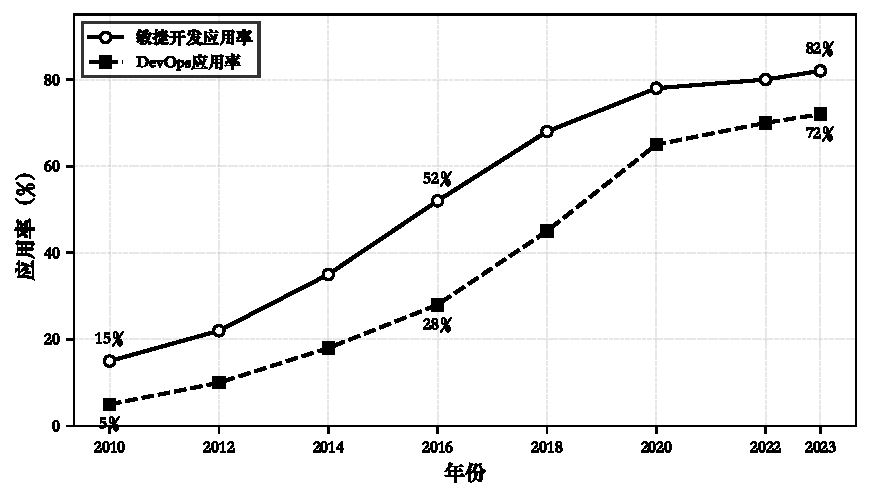
\includegraphics[width=0.85\textwidth]{myfigure/agile-adoption-rate.pdf}
\caption{中国互联网企业敏捷开发方法应用情况（2023）}
\label{fig:agile-adoption-rate}
\end{figure}

\subsection{DevOps实践的推广}

DevOps作为连接开发和运维的桥梁，在互联网公司得到了广泛实践。根据IDC的调研，2023年中国互联网企业DevOps实践普及率达到72\%，较2018年的35\%提升了一倍多\cite{idc2023agile}。通过持续集成（CI）、持续交付（CD）、自动化测试、基础设施即代码（IaC）等技术手段，DevOps实现了从代码提交到生产部署的自动化流程。

DevOps实践带来的效益可以用效率提升率来量化：

\begin{equation}
\eta_{\mathrm{improvement}} = \frac{T_{\mathrm{traditional}} - T_{\mathrm{DevOps}}}{T_{\mathrm{traditional}}} \times 100\%
\label{eq:efficiency-improvement}
\end{equation}

其中，$T_{\mathrm{traditional}}$为传统模式下的时间成本，$T_{\mathrm{DevOps}}$为采用DevOps后的时间成本。具体效益体现为：

\begin{itemize}
\item \textbf{部署频率提升}：从传统的每月1-2次提升至每周甚至每日多次部署，头部互联网公司日均部署次数可达数十次至上百次；
\item \textbf{交付周期缩短}：从需求提出到功能上线的平均时间从30-45天缩短至7-14天，效率提升$\eta = \frac{37.5-10.5}{37.5} \times 100\% = 72\%$；
\item \textbf{故障恢复时间减少}：平均故障恢复时间（MTTR）从4-8小时降至0.5-2小时；
\item \textbf{变更失败率降低}：生产环境变更失败率从15-20\%降至5-8\%；
\item \textbf{自动化率提升}：代码构建、测试、部署的自动化率从40\%提升至85\%以上\cite{idc2023agile}。
\end{itemize}

互联网公司建立了完善的DevOps工具链，包括：
\begin{itemize}
\item 代码管理工具：Git（使用率98\%）、GitLab（62\%）、GitHub（58\%）；
\item 自动化构建工具：Jenkins（使用率75\%）、GitLab CI（45\%）、GitHub Actions（38\%）；
\item 容器化技术：Docker（使用率88\%）、Kubernetes（72\%）；
\item 监控告警系统：Prometheus（使用率65\%）、Grafana（58\%）、自研监控系统（42\%）\cite{idc2023agile}。
\end{itemize}

DevOps文化的建立也推动了组织变革。开发和运维团队打破壁垒，形成更紧密的协作关系。调查显示，实施DevOps后，跨团队沟通效率提升45\%，技术债务偿还速度提升60\%，团队成员技能广度提升35\%\cite{mckinsey2023tech}。

\begin{table}[htbp]
\centering
\caption{DevOps实践前后关键指标对比}
\label{tab:devops-metrics-comparison}
\begin{tabular}{lccc}
\toprule
\textbf{指标} & \textbf{传统模式} & \textbf{DevOps模式} & \textbf{提升幅度} \\
\midrule
部署频率 & 每月1-2次 & 每周5-10次 & 10-20倍 \\
交付周期 & 30-45天 & 7-14天 & 缩短60-70\% \\
MTTR（故障恢复时间） & 4-8小时 & 0.5-2小时 & 缩短70-85\% \\
变更失败率 & 15-20\% & 5-8\% & 降低50-65\% \\
自动化率 & 40\% & 85\% & 提升112\% \\
\bottomrule
\end{tabular}
\end{table}

\begin{figure}[htbp]
    \centering
    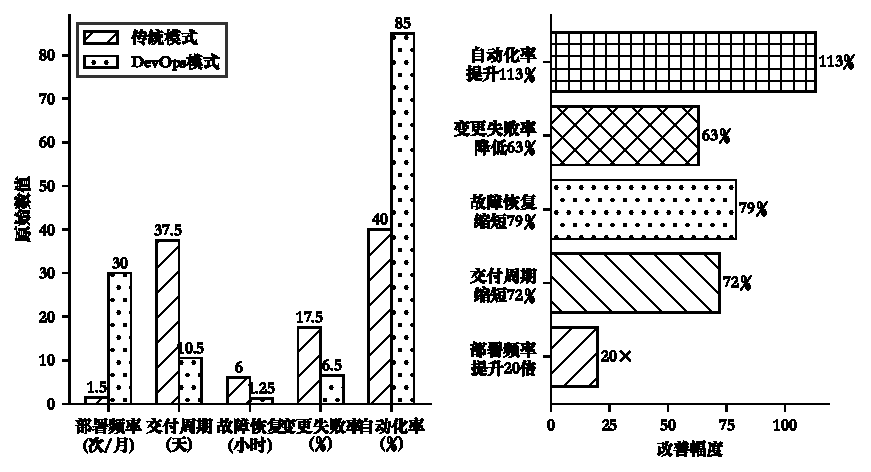
\includegraphics[width=0.95\textwidth]{myfigure/devops-metrics-comparison.pdf}
    \caption{DevOps实践前后关键指标对比与效益分析}
    \label{fig:devops-metrics-comparison}
\end{figure}

\subsection{创新激励机制的建立}

为了激发研发团队的创新活力，互联网公司建立了多元化的激励机制\cite{zhou2020positive,zhao2022diversity}。根据麦肯锡2023年调研，82\%的互联网企业建立了系统化的创新激励体系，较2018年的56\%大幅提升\cite{mckinsey2023tech}。

\textbf{物质激励方面}，实行具有竞争力的薪酬体系、股权激励计划、项目奖金等。根据智联招聘发布的《2024互联网行业人才流动与薪酬白皮书》：
\begin{itemize}
\item 2023年互联网行业研发人员平均年薪为26.8万元，同比增长3.5\%；
\item 核心技术岗位（如算法工程师、架构师）平均年薪达到35-50万元；
\item 58\%的互联网公司为核心研发人员提供股权或期权激励；
\item 项目奖金平均占年薪的15-25\%，头部企业可达30-40\%\cite{zhaopin2024tech}。
\end{itemize}

\textbf{精神激励方面}，提供技术晋升通道、给予技术自主权、营造创新氛围、举办技术交流活动等\cite{tang2022motivation,goh2022thriving}。调查显示：
\begin{itemize}
\item 92\%的大型互联网公司建立了技术和管理双通道晋升体系；
\item 平均每家公司每年举办内部技术分享会15-25场；
\item 68\%的公司支持员工参加外部技术会议并报销费用；
\item 45\%的公司设立了技术专家委员会，给予技术决策权\cite{mckinsey2023tech}。
\end{itemize}

许多互联网公司设立了内部创新项目，鼓励员工在工作之余探索新技术、开发新产品\cite{xu2011total}。例如，Google的20\%时间政策、3M的15\%规则等都是经典的创新激励机制。在中国互联网公司中，也出现了类似的实践\cite{gao2014open,zhang2008open}：
\begin{itemize}
\item 35\%的公司设立了创新时间制度（10-20\%工作时间）；
\item 52\%的公司设立了内部创新基金，平均规模为年度研发预算的8-12\%；
\item 48\%的公司举办内部创新大赛，获奖项目可获得10-50万元奖金和产品化支持；
\item 28\%的公司建立了内部孵化器，孵化周期为3-6个月\cite{idc2023agile}。
\end{itemize}

\begin{figure}[htbp]
\centering
% 注释：此处应插入图片文件 innovation-incentive-system.pdf
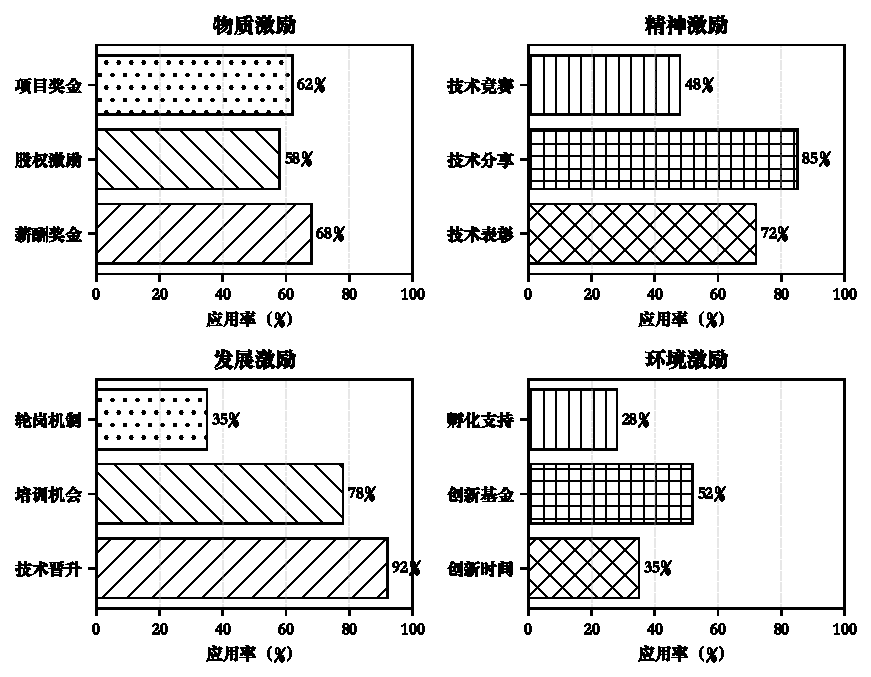
\includegraphics[width=0.85\textwidth]{myfigure/innovation-incentive-system.pdf}
\caption{互联网企业创新激励机制构成（2023）}
\label{fig:innovation-incentive-system}
\end{figure}

然而，激励机制的效果需要长期观察和持续优化。调查显示，虽然大多数企业建立了激励机制，但员工满意度仅为65\%，主要不满因素包括：晋升通道不够透明（58\%）、奖励标准不够公平（52\%）、创新失败缺乏包容（45\%）、长期激励不足（42\%）\cite{zhaopin2024tech}。

\subsection{技术平台与中台战略}

为了提升研发效率和技术复用率，互联网公司大力建设技术平台和中台体系\cite{wei2012excellence}。根据IDC的调研，2023年有65\%的大型互联网企业实施了中台战略，较2018年的28\%显著提升\cite{idc2023agile}。

技术中台包括数据中台、业务中台、技术中台等，通过将通用能力平台化、组件化，避免重复开发，提高响应速度，降低研发成本\cite{zhang2008open}。中台建设带来的效益：
\begin{itemize}
\item 代码复用率从平均25\%提升至60-70\%；
\item 新功能开发周期缩短30-40\%；
\item 系统稳定性提升，可用性从99.5\%提升至99.9\%以上；
\item 技术债务减少，维护成本降低25-35\%\cite{idc2023agile}。
\end{itemize}

阿里巴巴的"大中台、小前台"战略是典型代表\cite{xu2011total}。通过建设强大的中台能力，支撑前台业务的快速创新和灵活调整。这种架构模式在其他互联网公司也得到了借鉴和应用\cite{gao2014open}。技术平台的建设涉及架构设计、技术选型、团队组织、运营管理等多个方面\cite{pan2021transforming}。

中台战略的实施也面临挑战。调查显示，实施中台战略的企业中：
\begin{itemize}
\item 42\%认为"中台定位不清晰"是主要问题；
\item 38\%面临"中台与前台需求冲突"；
\item 35\%存在"中台响应速度慢"的问题；
\item 32\%难以"量化中台的价值贡献"\cite{idc2023agile}。
\end{itemize}

\section{当前环境下我国互联网企业研发管理面临的主要困境}

从宏观环境看，互联网行业面临多重外部压力的叠加。政策层面，监管趋严覆盖平台经济、数据安全与算法治理，合规成本上升\cite{cac2023internet}；经济层面，广告市场增速放缓、数字经济结构调整，叠加全球地缘政治不确定性，企业投资意愿收缩\cite{du2024mixed,li2022configuration}；技术层面，大模型等颠覆性技术快速迭代，技术路线选择风险加大\cite{li2024scientific,zheng2021disruptive}。竞争格局上，头部互联网企业在搜索、云计算、AI大模型等核心领域全面博弈，同时面临AI芯片供应受限（高端GPU依赖进口）、AI人才极度稀缺（供需比约1:10）的双重供给侧压力\cite{porter1980competitive}。上述宏观压力共同压缩了企业通过增量投入掩盖内部低效的空间，使以下结构性困境加速浮出水面。

\subsection{成本压力与资源约束}

经济下行环境下，互联网公司面临巨大的成本压力\cite{du2024mixed,li2022configuration}。根据中国网络空间研究院的数据，2022-2023年间，互联网行业整体营收增速放缓至7.6\%，但人力成本占营收比重从2020年的18.5\%上升至2023年的21.3\%\cite{cac2023internet}。

资本市场对盈利能力的要求提高，企业必须控制成本、提升效率。研发作为成本中心，成为降本增效的重点对象：
\begin{itemize}
\item 2022年有72\%的互联网企业缩减了研发预算，平均缩减幅度为15-20\%；
\item 项目优先级调整频繁，38\%的在研项目被暂停或取消；
\item 人员优化成为常态，2022-2023年累计裁员超过30万人，其中研发人员占45\%；
\item 外包比例提升，从2020年的12\%上升至2023年的18\%\cite{china100internet2023}。
\end{itemize}

资源约束下，企业需要在有限资源下实现最大价值。调查显示，研发管理面临的核心挑战：
\begin{enumerate}
\item \textbf{技术方向选择}（68\%的企业认为这是首要挑战）：在多个技术方向中如何选择，如何评估投入产出比；
\item \textbf{资源配置优化}（62\%）：如何在业务需求、技术创新、技术债务偿还之间平衡资源；
\item \textbf{研发效率提升}（56\%）：如何在人员减少的情况下保持或提升产出；
\item \textbf{团队士气维护}（52\%）：成本压力下如何保持团队积极性\cite{mckinsey2023tech}。
\end{enumerate}

成本压力也影响了团队士气。根据智联招聘的调研，2023年互联网研发人员的工作满意度为6.2分（10分制），较2020年的7.5分下降明显。主要不满因素包括：
\begin{itemize}
\item 工作强度增加：平均每周工作时间从48小时增至54小时（52\%）；
\item 晋升机会减少：2023年晋升率为8.5\%，较2020年的15.2\%大幅下降（48\%）；
\item 职业发展受限：担心技能提升机会减少（45\%）；
\item 薪酬增长放缓：2023年平均加薪幅度为3.5\%，远低于2020年的12.8\%（62\%）\cite{zhaopin2024tech}。
\end{itemize}

在这种环境下，企业容易陷入短视行为：过度关注短期收益，忽视长期技术储备；削减基础研究投入，影响核心竞争力培育；压缩人才培养预算，导致团队能力下降。如何在成本控制与创新发展之间找到平衡，是当前研发管理面临的重要课题。

上市公司年报数据为上述趋势提供了微观层面的佐证。表~\ref{tab:rd-investment-companies}已呈现主要互联网企业研发投入的绝对额变化；进一步计算可比口径下六家公司（阿里巴巴、百度、京东、拼多多、网易、哔哩哔哩）的加权平均研发增速：2021→2022年为$+1.0\%$，2022→2023年为$-3.0\%$，2023→2024年为$+14.5\%$，整体呈现先收缩后复苏的"V形"走势。其中，2022--2023年的收缩恰与行业"降本增效"周期高度吻合。值得注意的是，2024年的反弹主要由阿里巴巴（$+53.9\%$）和拼多多（$+33.6\%$）拉动，而百度（$-9.5\%$）、京东（$-0.6\%$）、携程（$-19.0\%$）等企业研发费用则仍处于收缩或平台期，表明头部企业在AI投入策略上已出现明显分化。

\subsection{人才流失、团队稳定与组织协作困境}

人才是互联网公司最重要的资产，也是研发管理的核心要素\cite{tang2022motivation,xu2024theoretical}。然而，当前互联网行业人才流动性显著增加。根据智联招聘2024年发布的数据\cite{zhaopin2024tech}：研发人员离职率为25.3\%（行业整体23.1\%），工作3--5年的研发人员离职率最高达29.8\%；主动离职占比62\%。主要原因依次为薪酬福利不满（68\%）、职业发展受限（58\%）、工作压力过大（52\%）、公司前景担忧（45\%）。

人才流失总成本可建模为：
\begin{equation}
TC = C_{\mathrm{recruit}} + C_{\mathrm{train}} + C_{\mathrm{prod\_loss}} + C_{\mathrm{know\_loss}}
\label{eq:turnover-cost}
\end{equation}
其中各项分别为招聘、培训、生产力损失和知识流失成本\cite{mckinsey2023tech}。综合影响包括：38\%的项目因核心成员离职而延期或质量下降；技术文档完整度平均仅60\%，知识传承困难；团队凝聚力持续下滑。

人才流失问题与组织协作困境相互强化。随着公司规模扩大，知识孤岛问题尤为突出：68\%的企业存在技术经验难以跨团队传播的问题；30--40\%的功能模块存在跨团队重复建设；跨部门协作障碍主要体现在沟通成本高（72\%企业反映约40\%跨团队会议低效）、目标不一致（58\%）、资源竞争（52\%）\cite{shen2024ecosystem,hoda2021socio}。企业虽尝试通过技术委员会、技术中台等方式破解孤岛，但效果有限——建立技术委员会的企业中仅38\%认为"有效推动了技术协同"，跨团队代码复用率平均仅15--20\%，远低于预期\cite{zimmermann2024strategies,developer2024experience}。这一现象的制度根源将在第四章百度案例中深入剖析。

\subsection{技术资产治理：技术负债积累与周转效率}

研发管理中，\textbf{技术资产}（TA）指可复用、可沉淀的技术能力与平台；\textbf{技术负债}（TD）指为短期进度妥协而积累的、需在后续以重构成本为代价偿还的欠账\cite{cunningham1993wycash,kruchten2012technical}。TD的动态累积过程可建模为：
\begin{equation}
TD_t = TD_{t-1} + \alpha \cdot N_t - \beta \cdot R_t + \gamma \cdot TD_{t-1}
\label{eq:tech-debt}
\end{equation}
其中$N_t$为新增债务，$R_t$为偿还量，$\gamma$为债务利息系数（旧债因系统演进增加维护难度）。当$\alpha N_t + \gamma TD_{t-1} > \beta R_t$时TD持续累积；其对研发效率的影响呈指数衰减：$E_t = E_0 \cdot e^{-\delta \cdot TD_t}$\cite{li2015systematic}。行业数据显示，技术债务占总研发成本的35--45\%，62\%的新功能开发受TD制约导致周期延长20--30\%\cite{idc2023agile}。

上述困境可归结为一个核心命题：大量研发投入是否真正转化为了可流转的技术资产？本文引入\textbf{技术资产周转率}（R\&D Capital Turnover）进行量化分析。技术资产存量采用永续盘存法估算\cite{hall1990rdcapital,lev1996capitalization}：
\begin{equation}\label{eq:rd-capital-stock}
K_t = (1 - \delta) \cdot K_{t-1} + RD_t
\end{equation}
技术资产周转率定义为$\text{营业收入}/K_t$。基于七家主要上市公司2019--2024年数据（图~\ref{fig:rd-capital-turnover}），核心发现为：\textbf{百度研发强度行业最高（16--20\%），但TA周转率长期最低且持续下滑}（1.31→1.12倍），是唯一持续下降的企业，说明研发投入更多沉积为技术库存而非商业价值——这一矛盾将在第四章深入剖析。京东（13.6倍）和拼多多（1.75→8.25倍）则展示了技术资产高效转化的路径。

\begin{figure}[htbp]
\centering
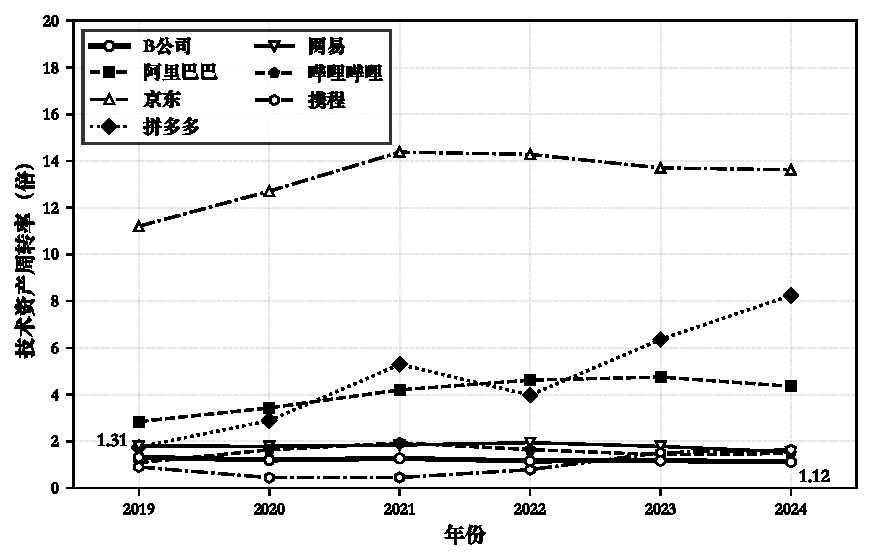
\includegraphics[width=\textwidth]{myfigure/rd-capital-turnover.pdf}
\caption{头部互联网企业技术资产运营效率分析（R\&D Capital Stock法，2019--2024）。数据来源：各公司年度财务报告；技术资产存量采用永续盘存法估算（$\delta=15\%$）。}
\label{fig:rd-capital-turnover}
\end{figure}

\section{生成式人工智能带来的新冲击}

2022年底ChatGPT的发布标志着人工智能进入生成式AI时代，这一技术变革正在对互联网公司的研发管理产生深远而系统性的影响\cite{storey2024disruptive}。生成式AI不仅改变了软件开发的技术手段，更重新定义了产品形态、组织能力和竞争格局，成为互联网公司研发管理面临的最重大挑战之一。

\subsection{AI辅助编程与研发范式变革}

AI辅助编程工具的快速普及正在重塑软件开发流程。根据GitHub 2024年开发者调查，全球已有超过100万开发者使用GitHub Copilot，92\%的开发者报告生产力有所提升\cite{github2024copilot}。代码生成效率提升30--50\%，调试时间缩短25--35\%，文档自动生成节省40--50\%时间。然而，58\%的企业反映AI生成代码存在质量隐患，42\%担心安全漏洞，过度依赖AI工具还可能导致代码一致性下降，加速技术负债积累\cite{iresearch2024ai}。

生成式AI时代同步要求研发人员具备全新技能组合：提示工程（65\%企业列为必备技能，但仅18\%人员掌握）、AI模型理解、人机协作能力、AI安全意识。72\%的企业缺乏系统的AI技能培训体系，年轻开发者（25--30岁）适应速度是资深开发者（35岁以上）的2--3倍，38\%的资深工程师面临技能贬值焦虑\cite{ccidconsulting2024ai}。

\subsection{产品形态、技术架构与战略选择}

生成式AI催生了全新的产品类别：对话式界面（百度文心一言、阿里通义千问等）、AI Agent、内容生成工具、智能决策系统。技术架构层面，大模型训练推理带来海量算力需求（单次训练成本数百万至数千万元）、响应时间优化（用户要求＜2秒）、API调用成本（每千次对话0.5--5元）等新挑战\cite{idc2024genai}。

企业面临"自研vs外购"的艰难战略选择：68\%的大型互联网企业采用"自研为主、外购为辅"的混合策略\cite{idc2024genai}。从已有数据可见头部企业AI策略的明显分化（表~\ref{tab:ai-rd-strategy}）——阿里（$+53.9\%$）、拼多多（$+33.6\%$）持续加码，百度（$-9.5\%$）研发总额略降但AI核心投入比重提升，京东、网易趋于稳健。这一格局将直接影响未来2--3年的技术竞争格局。

\subsection{AI人才竞争与伦理合规}

AI人才成为最稀缺资源：2023年AI领域人才缺口约100万人，供需比约1:10，算法工程师平均年薪50--80万元，顶尖人才达200--500万元，平均在职时长仅1.8年\cite{zhilian2024ai}。85\%的企业需要投入专门资源进行AI合规管理，《生成式人工智能服务管理暂行办法》（2023年8月）对AI服务提出明确要求，内容审核成本上升30--50\%，产品上线周期延长20--40\%\cite{idc2024genai,cyberspace2023genai}。

\subsection{AI冲击对技术资产管理的深层影响}

生成式AI的冲击不只是技术层面的挑战，更是技术资产治理逻辑的重构。AI工具大规模渗透后，原有的技术资产（基于规则和传统算法的工程积累）面临快速折旧风险，而新一代AI Native的技术资产（大模型、数据飞轮、Prompt工程体系）需要全新的生命周期管理逻辑。这意味着TA周转率的计算基准和折旧参数都需要随AI渗透程度动态调整——这也是本文第四章分析百度案例时的重要背景假设：百度当前TA周转率的低迷，部分原因正是旧有语音/搜索技术资产的折旧加速与新AI资产尚未形成商业闭环之间的过渡性摩擦。

生成式AI对组织逻辑的冲击，比技术层面的影响更为深远。笔者于2026年1月赴硅谷访问期间，观察到一个显著趋势：\textbf{当地绝大多数AI创业公司的团队规模控制在15人以内，且招聘偏好从"管理者/Leader"明显转向"超级IC（独立贡献者，Individual Contributor）"——企业所需要的不是能分配任务的人，而是能独当一面、直接产出高质量成果的超级个体。}这一现象绝非偶然。AI工具链大幅降低了分工协作的边际收益，同时极大放大了单个高能力个体的产出上限；在这一背景下，\textbf{组织规模的增长不再自动带来能力的增长，反而可能因沟通损耗和协调成本的非线性上升而稀释整体效能。}

这一趋势在国内同样有迹可循。\textbf{DeepSeek V3的发布在业界引发强烈震动：其背后数据团队仅约50人，整体研发规模不过百人，却产出了足以与国际顶级实验室竞争的大模型成果。}这一案例深刻动摇了"大模型必须依托大组织"的行业假设，也重新定义了"研发竞争力"的内涵——\textbf{高密度的超级IC团队配合先进AI工具链，其单位人效可能远超传统大规模分工团队。}对于正在推进研发组织转型的大型互联网企业而言，这意味着一个根本性的战略命题需要重新审视：\textbf{降本增效的解题方向，是"用更少的人做更多的事"，而非"用更多的人分摊更细的任务"。}这对百度等传统大厂的组织范式构成的挑战，将在第四章中结合具体案例深入分析。

\begin{table}[htbp]
\centering
\caption{头部互联网企业AI战略与研发投入动向（2024年）}
\label{tab:ai-rd-strategy}
\begin{tabular}{llrp{6cm}}
\toprule
\textbf{企业} & \textbf{AI战略方向} & \textbf{研发费用（亿元）} & \textbf{主要AI产品/布局} \\
\midrule
阿里巴巴 & 大模型全栈自研 & 588（$+53.9\%$） & 通义千问、百炼平台、AI云基础设施 \\
百度     & AI原生应用落地 & 219（$-9.5\%$）  & 文心一言、文心大模型4.0、AI搜索 \\
腾讯     & AI能力中台化   & 707（$+10.3\%$） & 混元大模型、AI助手、广告智能化 \\
拼多多   & AI赋能供应链   & 147（$+33.6\%$）& 搜推AI算法、农业AI、国际化AI能力 \\
京东     & AI工业化落地   & 163（$-0.6\%$） & 言犀大模型、智能仓储、AI客服 \\
网易     & AI内容创作     & 156（$-5.5\%$） & 子曰大模型、AI游戏NPC、AI翻译 \\
哔哩哔哩 & AI视频创作     & 47（$+4.4\%$）  & AI视频生成、AI弹幕分析、创作辅助 \\
\bottomrule
\multicolumn{4}{l}{\small 括号内为2023→2024财年增速；所有数据均以各公司年报``研发费用/研究及开发成本''科目为准，各公司财年截止日期略有差异。} \\
\multicolumn{4}{l}{\small 数据来源：各公司年度财务报告。}
\end{tabular}
\end{table}

从表~\ref{tab:ai-rd-strategy}可见，各企业的AI研发策略呈现明显分化：阿里和拼多多持续加码，体现出对AI投资回报的高预期；百度尽管研发总额略降，但其AI核心投入（文心大模型、智能云）比重持续提升；京东、网易则趋于稳健，侧重将AI能力向已有业务场景渗透，而非大规模新建基础模型。这一格局与各公司的市场地位、现金流状况、业务壁垒密切相关，也将直接影响未来2--3年的技术竞争格局。

图~\ref{fig:ai-rd-investment-2024}以水平柱状图形式更直观地呈现了上述分化格局，正增长（绿色）与负增长（红色）的鲜明对比凸显了头部企业在AI投入策略上的分歧。

\begin{figure}[htbp]
\centering
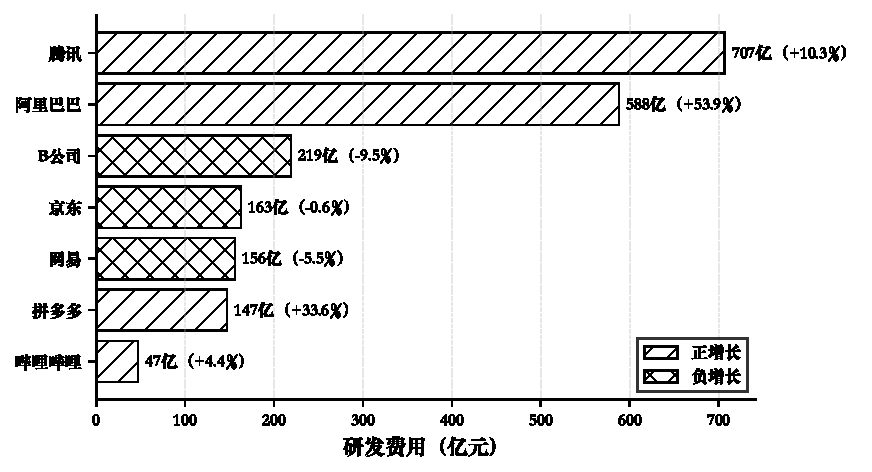
\includegraphics[width=0.92\textwidth]{myfigure/ai-rd-investment-2024.pdf}
\caption{头部互联网企业AI研发投入及增速（2024年）}
\label{fig:ai-rd-investment-2024}
\end{figure}

\begin{table}[htbp]
\centering
\caption{生成式AI对互联网研发管理的影响维度}
\label{tab:ai-impact-summary}
\begin{tabular}{p{2.5cm}p{4.5cm}p{5cm}}
\toprule
\textbf{影响维度} & \textbf{主要变化} & \textbf{关键数据} \\
\midrule
开发效率 & AI辅助编程工具普及 & 代码生成效率提升30-50\%，100万+开发者使用 \\
技能需求 & 提示工程等新技能 & 65\%企业列为必备，但仅18\%人员掌握 \\
产品形态 & AI Native产品涌现 & 对话式AI、智能助手成为主流 \\
技术架构 & 大模型训练推理 & 单次训练成本数百万至千万元 \\
战略选择 & 自研vs外购 & 68\%采用混合策略 \\
人才竞争 & AI人才极度稀缺 & 缺口100万，供需比1:10，年薪50-80万 \\
伦理合规 & 新监管要求 & 85\%企业需专门合规资源，周期延长20-40\% \\
\bottomrule
\end{tabular}
\end{table}

\begin{table}[htbp]
\centering
\caption{中国互联网企业研发管理主要困境汇总（2023-2024）}
\label{tab:challenges-summary}
\begin{tabular}{p{2.5cm}p{4cm}p{5cm}}
\toprule
\textbf{困境类别} & \textbf{核心问题} & \textbf{主要数据指标} \\
\midrule
成本压力 & 降本增效、资源约束 & 研发投入增速降至5.3\%，裁员30万人 \\
人才流失 & 团队稳定性下降 & 离职率25.3\%，工作满意度6.2/10分 \\
创新困境 & 技术债务、创新速度 & 技术债务占成本35-45\%，创新周期需30天内 \\
组织协作 & 知识孤岛、跨部门协作 & 重复开发30-40\%，跨团队复用率仅15-20\% \\
远程协作 & 分布式团队管理 & 52\%混合办公，沟通效率降低15-25\% \\
技术变革 & AI浪潮冲击 & 62\%难以跟上AI发展，56\%缺乏AI经验 \\
\bottomrule
\end{tabular}
\end{table}

为更直观地呈现各类困境之间的优先级关系，图~\ref{fig:challenges-quadrant}将上述六类困境按"重要性"与"紧迫性"两个维度进行四象限定位。成本压力与AI技术变革同时落入"高重要/高紧迫"象限，是当前研发管理最迫切需要应对的挑战；技术债务与组织协作问题则属于"高重要/中紧迫"区域，需要纳入中长期系统改善计划。

\begin{figure}[htbp]
\centering
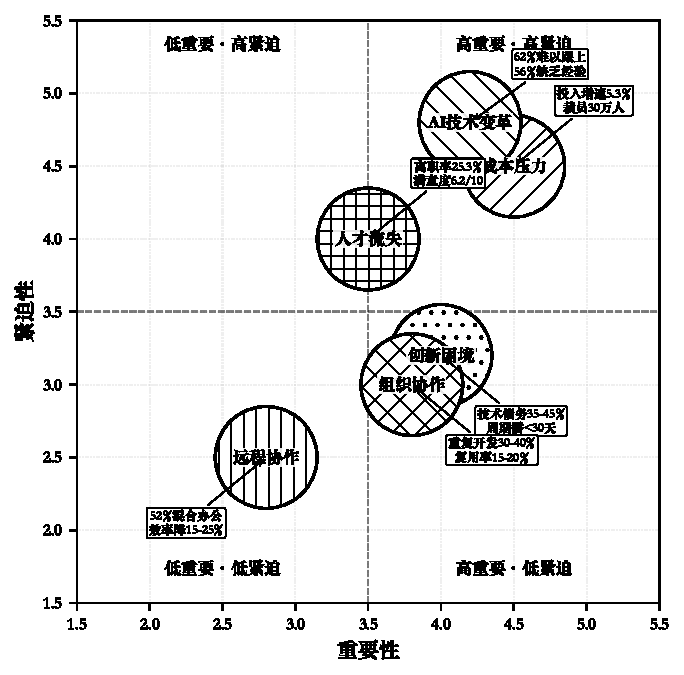
\includegraphics[width=0.88\textwidth]{myfigure/challenges-quadrant.pdf}
\caption{中国互联网企业研发管理主要困境分布（2023--2024）}
\label{fig:challenges-quadrant}
\end{figure}

\section{本章小结}

本章系统分析了我国互联网公司研发管理的发展历程、主要实践和当前困境，通过大量量化数据和图表展示了行业发展的真实状况。

从早期探索（2000-2010）到快速扩张（2010-2020），再到当前的转型调整（2020至今），研发管理模式经历了深刻变革。数据显示，中国互联网网民规模从2000年的0.23亿增长至2020年的9.86亿，互联网企业研发人员从约5万增长至超过150万，研发投入占比从8\%提升至20\%，显示出行业的快速发展。

在研发管理方法方面，敏捷开发应用率达到82\%，DevOps实践普及率达到72\%，技术中台战略实施率达到65\%。这些先进管理方法的应用使产品上线周期缩短40-50\%，部署频率提升10-20倍，研发效率显著提升。

\textbf{困境的系统性归因}：然而，当前互联网企业研发管理面临的多重挑战——成本压力、人才流失、技术债务积累、创新停滞——并非孤立的偶发事件，而是三层相互强化的结构性力量共同作用的结果，在特定历史节点集中爆发。

第一层是\textbf{外部环境的周期性收紧}：宏观经济下行、资本市场从"增长逻辑"切换到"盈利逻辑"、大模型技术颠覆性冲击同步到来——三种外部压力在2022-2023年同期叠加，压缩了企业通过增量投入掩盖内部低效的空间，迫使深层矛盾浮出水面。这一层是触发器，但不是根因。

第二层是\textbf{组织形态与业务复杂度的历史错配}：快速扩张期以"人海战术"和"职能分工"为主体搭建的研发组织，在业务收缩、AI重构研发范式的新阶段，其高协作成本和低响应速度的结构性缺陷被放大。技术债务的积累正是这种错配在工程层面的积累——每一次"先跑通再优化"的快速迭代决策，都是在未来的效率账单上签字。这一层是存量包袱。

第三层也是最隐蔽的一层，是\textbf{内部制度激励的系统性扭曲}：短期KPI压力、成本分摊为导向的内部结算机制、以资历而非贡献为核心的晋升体系，共同将"维护存量"的激励置于"创造增量"之上。当员工发现精耕细作的技术资产积累不如快速完成内部结算指标获益更大时，研发文化的退化便难以逆转。这一层是内因，也是本研究重点关注的改进对象。

三层结构相互强化——外部压力触发对内部低效的追问，历史包袱放大了外部冲击的破坏力，而制度扭曲则阻断了组织通过学习与调整自我修复的能力。这正是为什么互联网行业的当前困境不是一个可以通过局部优化解决的管理问题，而是需要"组织—流程—激励—制度"四维协同变革的系统性挑战。

值得注意的是，上述困境并非所有互联网公司都以同等程度呈现——部分企业已在组织转型上率先探索，而另一些企业则深陷"结构未动、制度先僵"的困局。百度公司的特殊性在于：其历经了从搜索巨头到AI战略转型的完整路径，TPG向BMU/AMU架构的调整是国内规模最大、影响面最广的产品型组织转型案例之一，且因有内部视角可供深度观察，能够揭示公开财报数据之下的制度运作逻辑。因此，下一章将以百度为分析对象，深入诊断其研发管理实践中"结构调整≠效能提升"的深层原因，为互联网公司研发管理转型提供可借鉴的经验与教训。

</invoke>
